\documentclass{beamer}
\usepackage{listings}
\lstset{
%language=C,
frame=single, 
breaklines=true,
columns=fullflexible
}
\usepackage{blkarray}
\usepackage{subcaption}
\usepackage{url}
\usepackage{xurl}
\usepackage{tikz}
\usepackage{mathrsfs}
\usepackage{tkz-euclide} % loads  TikZ and tkz-base
%\usetkzobj{all}
\usetikzlibrary{calc,math}
\usepackage{float}
\newcommand\norm[1]{\left\lVert#1\right\rVert}
\renewcommand{\vec}[1]{\mathbf{#1}}
\usepackage[export]{adjustbox}
\usepackage[utf8]{inputenc}
\usepackage{amsmath}
\usepackage{amssymb}
\usepackage{bm}
\usepackage{tikz}
\usetikzlibrary{automata, positioning}
\usetheme{Boadilla}
\providecommand{\pr}[1]{\ensuremath{\Pr\left(#1\right)}}
\providecommand{\sbrak}[1]{\ensuremath{{}\left[#1\right]}}
\providecommand{\lsbrak}[1]{\ensuremath{{}\left[#1\right.}}
\providecommand{\rsbrak}[1]{\ensuremath{{}\left.#1\right]}}
\providecommand{\pr}[1]{\ensuremath{\Pr\left(#1\right)}}
\providecommand{\brak}[1]{\ensuremath{\left(#1\right)}}
\providecommand{\lbrak}[1]{\ensuremath{\left(#1\right.}}
\providecommand{\rbrak}[1]{\ensuremath{\left.#1\right)}}
\providecommand{\cbrak}[1]{\ensuremath{\left\{#1\right\}}}
\providecommand{\lcbrak}[1]{\ensuremath{\left\{#1\right.}}
\providecommand{\rcbrak}[1]{\ensuremath{\left.#1\right\}}}

\title{Research Paper Presentation}
\author{Nelakuditi Rahul Naga - EE20BTECH11036}
\date{June 19, 2021}

\begin{document}

\begin{frame}
\titlepage
\end{frame}

\begin{frame}
    \begin{block}{Title}
    UAV Communication Strategies in the Next Generation of Mobile Networks.
    \end{block}
    \begin{block}{Authors}
    \begin{itemize}
        \item Hamed Hellaoui, Miloud Bagaa - Communications and Networking Department, Aalto University, Finland.
        \item Ali Chelli,Faculty of Engineering and Science, University of Adger, Norway.
        \item Tarik Taleb, Communications and Networking Department,University of Oulu, Finland.
    \end{itemize}
    \end{block}
    \begin{block}{Year of publication}
    2020.
    \end{block}
\end{frame}

\begin{frame}{}
\begin{block}{Abstract}
\begin{itemize}
    \item The Next Generation of Mobile Networks (NGMN) alliance advocates the use of different means to support vehicular communications to cope with the massive data generated by these devices which could affect Quality of Service (QoS).
    \item Hence, we propose efficient communication strategies for Unmanned Aerial Vehicles (UAVs).We also consider UAV-to-UAV scheme (U2U) to transmit data via relay UAVs in addition to the direct UAV-to-Infrastructure communications (U2I).
    \item The goal is to select for each UAV the best communication strategy ensuring the best QoS and the relay node to maximize the spectral efficiency.
    \item Finally, performance evaluations are conducted for different strategies to check the effectiveness of the proposed solution.
\end{itemize}
\end{block}
\end{frame}

\begin{frame}{Introduction}
\begin{itemize}
    \item UAVs have initiated a vast range of applications in different fields. They are predicted to achieve a significant expansion in the coming years.This will put a high pressure on the network infrastructure used for UAVs communication.
    \item UAV-enabled applications are of critical nature and require signaling messages that are sent with high data rate.This burden could result in decreased QoS for the associated applications and could also affect the overall operations of the UAVs.
    \item It is highly important to ensure an efficient communication infrastructure to accommodate the huge number of UAVs, along with their massive generated data in order to enable the adoption of UAVs in the future.
\end{itemize}
\end{frame}

\begin{frame}{}
 \begin{itemize}
     \item In this regard, both industrial and scientific communities are heading towards \textbf{using mobile networks as a key enabler for UAV communications} enabling UAVs to benefit from the advances achieved by these networks.
     \item The consideration of such an approach for UAVs will provide huge opportunity which can be exploited to cope with the burden associated with the UAV's massive data. This must be associated with efficient strategies to select the optimal communication mean for each UAV in a way to maximize the QoS.
     \item Different works by the industrial and academic communities studied   the challenges related to the use of cellular networks as a communication infrastructure for UAVs. However, the issue of communication strategies was not considered by these works dealing with mobile network-enabled UAVs.
 \end{itemize}   
\end{frame}

\begin{frame}{System Model and Problem Formulation}
  \begin{itemize}
      \item We consider in the proposed model most of propagation phenomena experienced by wireless signals,such as fast fading,path loss and interference. We derive the expression of the effective rate for the different communication strategies.
      \item We consider an uplink scenario in which UAVs send data to their serving base stations (BSs) using one of the following strategies :
      \end{itemize}
      \begin{block}{Different types of strategies}
        \begin{itemize}
            \item Strategy 1 : UAV sends its packet using a \textbf{Direct Communication} with its serving BS.
            \item Strategy 2 : The UAV uses \textbf{Dual Hop Communication} to transmit its data to the BS via a relay mode. This UAV operates in a decode and forward mode.
         \end{itemize}
      \end{block}
\end{frame}

\begin{frame}{}
 The schematic model for the above mentioned strategies can be observed below.
\begin{figure}[!ht]
    \centering
    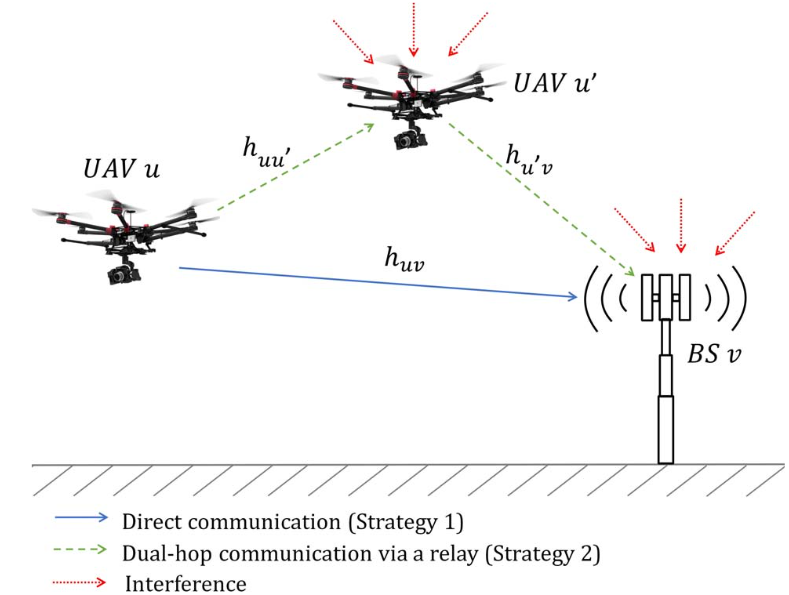
\includegraphics[scale=0.4]{rp6_Fig_1.png}
    \caption{System Model (Uplink Scenario)}
    \label{fig:System Model}
\end{figure}
\end{frame}

\begin{frame}{}
The notations we are going to use further on are represented in the following table:
\begin{table}[h]
\caption{Summary of Notations}
\centering
\begin{tabular}{|p{0.2\columnwidth}|p{0.7\columnwidth}|}
\hline
 \textbf{Notation} & \textbf{Description}\\
\hline
$\mathbb{U}$ & Set of UAVs.\\
\hline
$\mathbb{V}$& Set of BSs.\\
\hline
$uv$  & Link between a UAV $u \in \mathbb{U}$ and its serving BS $v \in \mathbb{V}$.\\
\hline
$uu^\prime$ & Link between a UAV $u \in \mathbb{U}$ and its relaying UAV $u^\prime \in \mathbb{U}$.\\
\hline
$\eta(u)$ & The neighbors of UAV $u$ in the graph $G$.\\
\hline
$X_{u,y}$ & A boolean variable that indicates whether UAV $u \in \mathbb{U}$ selects $y \in \eta(u)$ as the next hop.\\
\hline
$\varepsilon$ & A variable that represents the minimum effective rate in the network.\\
\hline
\end{tabular}
\label{table:1}
\end{table}
\end{frame}

\begin{frame}{}
In the figure \ref{fig:System Model} shown above :
\begin{itemize}
    \item $h_{uu^\prime}$,$h_{u^\prime v}$ and $h_{uv}$ are the fading coefficients for the links $uu^\prime$,$u^\prime v$ and $uv$ respectively which follow the \textbf{Nakagami-m distributions.}
    \item Both the relay UAV $u^\prime$ and destination BS $v$ are affected by several interferers. This interference originates from other UAVs in neighboring cells that use the same subcarriers as the source UAV $u$ and the relay UAV $u^\prime$.
\end{itemize}
\begin{block}{Nakagami-m Distribution}
The Nakagami-m distribution is a probability distribution related to the gamma distribution.It has two parameters :
\begin{enumerate}
\item A shape parameter $m$ (or $\mu) \geq \frac{1}{2}$.
\item A spread controlling parameter $\Omega$ (or $\omega)> 0$.
\end{enumerate}
\end{block}
\end{frame}

\begin{frame}{}
The PDF of the Nakagami-m distribution is shown below:
\begin{figure}[!ht]
    \centering
    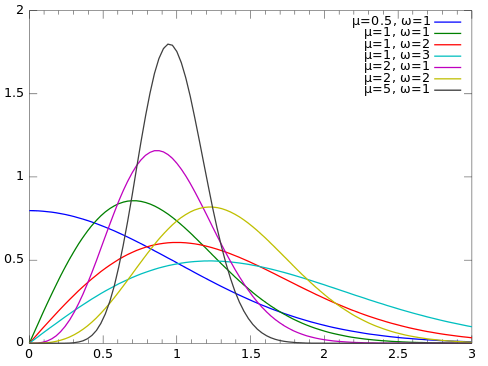
\includegraphics[scale=0.5]{rp6_Fig_2.png}
    \caption{PDF}
    \label{fig:PDF}
\end{figure}
\end{frame}

\begin{frame}{}
 The CDF of the Nakagami-m distribution is shown below:
 \begin{figure}[!ht]
    \centering
    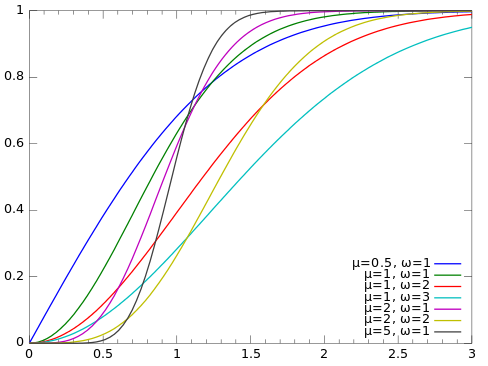
\includegraphics[scale=0.5]{rp6_Fig_3.png}
    \caption{CDF}
    \label{fig:CDF}
\end{figure}  
\end{frame}

\begin{frame}{}
 \begin{itemize}
     \item We assume that each interference term follows a Nakagami-m distribution. By adjusting the parameters of this distribution,we can model LOS (Line of Sight) and non-LOS conditions.
     \item Let $u \in \mathbb{U}$ denotes the transmitting UAV and $y \in \mathbb{U} \cup \mathbb{V}$ the receiving node. Then the recieved signal $r_{y}$ can be expressed as
     \begin{align}
         r_{y} = h_{uy}\sqrt{P_{u}}x_{u} + \sum_{t=1}^{N}h_{ty}\sqrt{P_{t}}x_{t} + n_{y}\label{eq:1}
     \end{align}
 where $h_{uy}$ refers to the channel gain between the transmitter $u$ and the receiver $y$.The second term in the RHS of equation \eqref{eq:1} accounts for the interference impact from node $t (t=1,2,...,N)$ and $h_{ty}$ refers to the fading coefficient from the interfering node $t$ to the receiver node $y$.The nodes $u$ and $t$ transmit the symbols $x_{u}$ and $x_{t}$ with the powers $P_{u}$ and $P_{t}$ respectively.
 \end{itemize}  
\end{frame}

\begin{frame}{}
   \begin{itemize}
       \item The third term in the RHS of equation \eqref{eq:1}, $n_{y}$, is a zero-mean additive white Gaussian noise with variance $N_{0}$. The instantaneous received \textbf{signal-to-noise ratio (SNR)},$\gamma_{uy}$,can be expressed as
       \begin{align}
         \gamma_{uy} = \frac{P_{u}h_{uy}^2}{N_{0}}\label{eq:2}
       \end{align}
       \item The mean value of $\gamma_{uy}$ is denoted by $\bar{\gamma}_{uy}$ and can be determined as
       \begin{align}
         \bar{\gamma}_{uy} =  \frac{P_{u}\mathbb{E}[h_{uy}^2]}{N_{0}} = P_{u} \times \frac{10^\frac{-PL_{uy}}{10}}{N_{0}}\label{eq:3}
       \end{align}
       where $\mathbb{E}[h_{uy}^2]$ represents the channel variance. $\mathbb{E}[.]$ denotes the expectation operator. The channel variance can be computed as $\mathbb{E}[h_{uy}^2] = 10^\frac{-PL_{uy}}{10}$ where $PL_{uy}$ represents the path loss in dB scale.
   \end{itemize} 
\end{frame}

\begin{frame}{}
 \begin{itemize}
     \item We now consider the path loss model adopted by 3rd Generation Partnership Project(3GPP) i.e.,
     \begin{align}
         PL_{uy} = 28.0 + 22\log_{10}(d^{3D}_{uy}) + 20\log_{10}(f_{c})\label{eq:4}
     \end{align}
     where $f_{c}$ stands for the carrier frequency, $d^{3D}_{uy}$ is the Euclidean distance between the transmitter and the receiver.
     \item Henceforth we use the shorthand notation $X \sim 
       \mathscr{G}(\alpha,\beta)$ to denote that $X$ follows a Gamma distribution with parameters $\alpha$ and $\beta$. The SNR $\gamma_{uv}$ is Gamma distributed with parameters $\alpha_{uv}$ and $\beta_{uv} = \dfrac{\bar{\gamma}_{uv}}{\alpha_{uv}}$ i.e; $\gamma_{uv} \sim \mathscr{G}(\alpha_{uv},\beta_{uv})$.
       \item The BS $v$ is affected by $N$ interfering nodes $t(t=1,2,...,N)$.The total interference at the BS is given by
       \begin{align}
    \gamma_{Iv} = \sum_{t=1}^{N}P_{t}h_{tv}^2 = \sum_{t=1}^{N}\gamma_{Itv}\label{eq:5}
       \end{align}
 \end{itemize}   
\end{frame}

\begin{frame}{}
\begin{itemize}
    \item The total interference at the BS in equation \eqref{eq:5} is the sum of $N$ independent non-identically distributed Gamma RV, with $\gamma_{Itv} \sim \mathscr{G}(\alpha_{tv},\beta_{tv})$.
    \item The PDF of total interference $\gamma_{Iv}$ can be approximated by a Gamma distribution with parameters $\alpha_{s}$ and $\beta_{s}$ i.e., $\gamma_{Iv} \sim \mathscr{G}(\alpha_{s},\beta_{s})$.The parameters $\alpha_{s}$ and $\beta_{s}$ can be expressed as follows
    \begin{align}
        \alpha_{s} &= \dfrac{(\sum_{t=1}^{N_{v}}\alpha_{tv}\beta_{tv})^2}{\sum_{t=1}^{N_{v}}\alpha_{tv}\beta_{tv}^2}\label{eq:6}\\
        \beta_{s} &= \dfrac{\sum_{t=1}^{N_{v}}\alpha_{tv}\beta_{tv}^2}{\sum_{t=1}^{N_{v}}\alpha_{tv}\beta_{tv}}\label{eq:7} 
    \end{align}
    where $\beta_{tv} = \dfrac{\bar{\gamma}_{tv}}{\alpha_{tv}}$.
\end{itemize}
\end{frame}

\begin{frame}{}
 \begin{itemize}
     \item In order to evaluate the the link quality between a UAV and the receiving BS,the expressions of the effective rate in the two strategies are given below
 \end{itemize}   
 \begin{block}{\textbf{Effective rate for Direct Communication}}
 For a UAV $u \in \mathbb{U}$ transmitting with a rate $R$ via a direct communication to its serving BS $v \in \mathbb{V}$, the effective rate at the receiving BS can be expressed as
 \begin{align}
 R^{uv}_{\text{eff}}(R) = R \times I(2^R-1,\alpha_{uv},\beta_{uv},\alpha_{s},\beta_{s})\label{eq:8}
 \end{align}
 The function $I(2^R-1,\alpha_{uv},\beta_{uv},\alpha_{s},\beta_{s})$ or $I(.)$ can be expressed as 
 \begin{align}
   I(.)= (\dfrac{x\beta_{s}}{\beta})^{-\alpha_{s}}\dfrac{\Gamma(\alpha+\alpha_{s})}{\Gamma(\alpha)\Gamma(1+\alpha_{s})}{}_{2}F_{1}(\alpha_{s},\alpha + \alpha_{s},1+\alpha_{s},\dfrac{-\beta}{x\beta_{s}})\label{eq:9}
 \end{align}
 where $\Gamma(.)$ is the Gamma function and ${}_{2}F_{1}(a,b,c,z)$ is the \textbf{Gauss Hypergeometric Function}.
 \end{block}
 
\end{frame}

\begin{frame}{}
\begin{block}{\textbf{Effective Rate for Dual-Hop Communication}}
 For a UAV $u \in \mathbb{U}$ transmitting with a rate $R$ via a relay UAV $u^\prime$  the effective rate at the receiving BS $v \in \mathbb{V}$ can be expressed as
 \begin{align}
 R^{u}_{\text{eff}}(R) = R \times I(2^R-1,\alpha_{uu^\prime},\beta_{uu^\prime},\alpha_{s_{u^\prime}},\beta_{s_{u^\prime}}) \times I(2^R-1,\alpha_{u^\prime v},\beta_{u^\prime v},\alpha_{s},\beta_{s})\label{eq:10}
 \end{align}
 The total interference at the relay UAV $u^\prime$ and the BS $v$ are approximated by the Gamma distributions $\mathscr{G}(\alpha_{s_{u^\prime}},\beta_{s_{u^\prime}})$ and $\mathscr{G}(\alpha_{s},\beta_{s})$ respectively.
\end{block}

 \begin{block}{Proof for equations \eqref{eq:8}, \eqref{eq:9} and \eqref{eq:10}}
 \url{https://github.com/gadepall/papers/blob/master/Research-papers-2/rp6.pdf}
 \end{block} 
\end{frame}

\begin{frame}{}
 \begin{block}{Gauss Hypergeometric Function}
 It is defined as 
 \begin{align}
 {}_{2}F_{1}(a,b,c,z) = \sum_{n=0}^{\infty}\dfrac{(a)_{n}(b)_{n}}{(c)_{n}}\dfrac{z^n}{n!} \ \text{if}\ \vert{z}\vert < 1\nonumber
 \end{align}
 where 
 \begin{align}
(q)_{n}  = 
\begin{cases}
1 & n=0
\\
q(q+1)...(q+n-1) & n > 0
\end{cases} \nonumber
\end{align}
 \end{block}   
\end{frame}

\begin{frame}{UAV Communication Optimal Strategies}
 \begin{itemize}
     \item In order to enhance the effective rate, an optimal selection of the communication strategy and the next hop should be achieved for each cellular-enabled UAV in the network.
     \item In order to simplify the problem , we reduce the search space of next hop of a UAV $u$ to a feasible set $\eta(u)$.We define a range $\bar{d}_{u}$ for each UAV $u$ and introduce the following lemma
 \end{itemize} 
 \begin{block}{Lemma}
 A UAV $u \in \mathbb{U}$ can transmit its packets to a next node $y \in \mathbb{U} \in \mathbb{V}$ iff the Euclidean distance between the nodes is within a range of $\bar{d}_{u}$ defined as
 \begin{align}
 \bar{d}_{u} = 10^{\dfrac{-[10\log_{10}(\dfrac{\gamma_{th}N_{0}}{P_{u}}) + 28.0 + 20\log_{10}(f_{c})]}{22}}\label{eq:11}
 \end{align}
 where $\gamma_{th}$ is the threshed SNR which reflects the sensitivity of the server.
 \end{block}
\end{frame}

\begin{frame}{}
\begin{block}{Proof of Lemma}
From the equations \eqref{eq:3} and \eqref{eq:4} we have
\begin{align}
\bar{\gamma}_{uy} = \dfrac{P_{u}}{N_{0}} \times 10^{-\dfrac{28.0 + 22\log_{10}(d^{3D}_{uy}) + 20\log_{10}(f_{c})}{10}}\label{eq:12}
\end{align}
In general, a packet is successfully received if the mean SNR at y, $\bar{\gamma}_{uy}$, exceeds the threshold $\gamma_{th}$. Thus we can derive $\bar{d}_{u}$ from equation \eqref{eq:12} as follows
\begin{align}
 \bar{d}_{u} = 10^{\dfrac{-[10\log_{10}(\dfrac{\gamma_{th}N_{0}}{P_{u}}) + 28.0 + 20\log_{10}(f_{c})]}{22}}\nonumber
 \end{align}
  which is same as equation \eqref{eq:11}. Hence, proved.
\end{block}    
\end{frame}

\begin{frame}{}
\begin{itemize}
\item Based on the communication range $\bar{d}_{u}$ of each UAV $u$, we define the set $\eta(u)$ of $u$'s neighbors as follows
  \begin{align}
      \eta(u) = \{u^\prime \in \mathbb{U};d^{3D}_{uu^\prime} \leq \bar{d}_{u}\} \cup \{v\}\label{eq:13}
  \end{align} 
 \item The set $\eta(u)$ gathers the UAVs having an euclidean distance less than $ \bar{d}_{u}$ to the UAV $u$. We also assume that the serving BS $v$ is among the neighbors of UAV $u$.
 \item To find the optimal strategy to be selected by each UAV we model the problem as an integer program. We define a Boolean variable $X_{u,y}$ as shown in table \ref{table:1}.This variable is also used to ensure that each UAV is connected to a BS with at most two hops.
 \item The formulation of the problem is as follows
 \begin{align}
 \text{max}\, \underset{u\in \mathbb{U}}{\text{min}}(\sum_{y\in \eta(u)}X_{u,y}R^{u}_{\text{eff}}(R))\label{eq:14}
 \end{align}
 i.e., to maximize the minimum effective rate for the set $\mathbb{U}$ of UAVs.
 \end{itemize}
 \end{frame}

\begin{frame}{}
The following constraints are to be satisfied in addition to equation \eqref{eq:14} 
\begin{align}
 \forall{u} \in \mathbb{U},\forall{y} \in \eta(u);\ X_{u,y} \in \{0,1\}\label{eq:15}
 \end{align}
\begin{align}
   \forall{u} \in \mathbb{U};\sum_{y\in \eta(u)}X_{u,y} = 1\label{eq:16}
\end{align}  
\begin{align}
    \forall{u} \in \mathbb{U};\ \Bigg(\sum_{y \in \eta(u) \cap \mathbb{U}}X_{u,y}\Bigg) \times \Bigg(\sum_{z \in \eta(y) \cap \mathbb{U}}X_{y,z}\Bigg) = 0\label{eq:17}
\end{align}
\begin{itemize}
    \item Constraint \eqref{eq:15} limits the value of decision variable $X_{u,y}$ to $\{0,1\}$.
    \item Constraint \eqref{eq:16} ensures that each UAV $u$ will select only one neighbor as successor.
    \item Constraint \eqref{eq:17} ensures that the communication between a UAV to a BS will go through at most two hops.
\end{itemize}
\end{frame}

\begin{frame}{}
\begin{itemize}
    \item However the optimization problem is not convex due to constraint \eqref{eq:17}.Therefore to simplify this constraint and make the problem linear, we propose the following transformation
    \begin{align}
    \forall{u} \in \mathbb{U};\ \sum_{y \in \eta(u) \cap \mathbb{U}}X_{y,u} \leq \Bigg(1- \sum_{z \in \eta(u) \cap \mathbb{U}}X_{u,z}\Bigg)(\vert{\eta(u)}\vert - 1)\label{eq:18}
    \end{align}
    \item Equation \eqref{eq:18} ensures that if a UAV $u$ selects another UAV $z$ as a relay node, the former is not selected by any other UAV $y$ for relaying packets.
    \item In order to implement the max-min problem, we introduce $\varepsilon$ (defined in table \ref{table:1}). The following condition is therefore considered
    \begin{align}
       \forall{u} \in \mathbb{U};\ \varepsilon \leq  \sum_{y \in \eta(u)} X_{u,y}R^{u}_{\text{eff}}(R)\label{eq:19}
    \end{align}
\end{itemize}    
\end{frame}

\begin{frame}{}
\begin{itemize}
    \item The previous model can now be updated as follows
\end{itemize}
\begin{align}
\text{max}\ \varepsilon
\end{align}
\qquad  \textbf{s.t.}
\begin{align}
       \forall{u} \in \mathbb{U};\ \varepsilon \leq  \sum_{y \in \eta(u)} X_{u,y}R^{u}_{\text{eff}}(R)\label{eq:21}
\end{align}
\begin{align}
 \forall{u} \in \mathbb{U},\forall{y} \in \eta(u);\ X_{u,y} \in \{0,1\}\label{eq:22}
\end{align}
\begin{align}
   \forall{u} \in \mathbb{U};\sum_{y\in \eta(u)}X_{u,y} = 1\label{eq:23}
\end{align}
\begin{align}
    \forall{u} \in \mathbb{U};\ \sum_{y \in \eta(u) \cap \mathbb{U}}X_{y,u} \leq \Bigg(1- \sum_{z \in \eta(u) \cap \mathbb{U}}X_{u,z}\Bigg)(\vert{\eta(u)}\vert - 1)\label{eq:24}
\end{align}
\end{frame}

\begin{frame}{Performance Evaluation}
\begin{itemize}
    \item As can be seen from figure \ref{fig:Receiver Sensitivity} shown below ,decreasing the value of the parameter $\gamma_{th}$ allows enhancing the effective rate at the BSs. This is due to the fact that the smaller $\gamma_{th}$ is the better the receiver can detect weaker signals.
\begin{figure}[!ht]
    \centering
    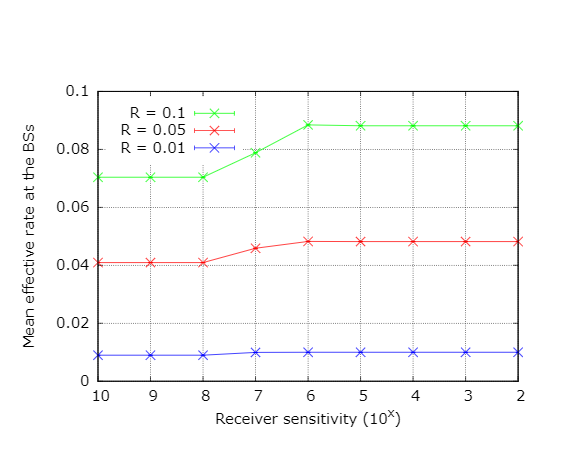
\includegraphics[scale=0.4]{rp6_Fig_4.png}
    \caption{Effect of receiver sensitivity $\gamma_{th}$ at different transmission rates R}
    \label{fig:Receiver Sensitivity}
\end{figure}
\end{itemize}
\end{frame}

\begin{frame}{}
 \begin{itemize}
     \item As can be seen from figure \ref{fig:Effective Rate} shown below , the proposed solution achieves better effective rate when considering different number of deployed UAVs.The proposed solution achieves better QoS even for a large number of UAVs i.e., even when the interference is high.
 \end{itemize}
 \begin{figure}[!ht]
    \centering
    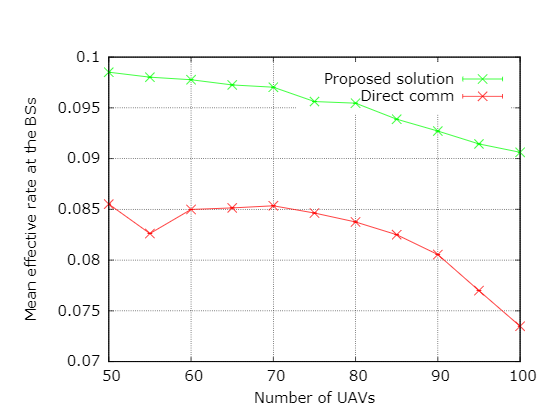
\includegraphics[scale=0.4]{rp6_Fig_5.png}
    \caption{Evaluation of the effective rate at the BSs}
    \label{fig:Effective Rate}
\end{figure} 
\end{frame}

\begin{frame}{}
\begin{itemize}
    \item The number of UAVs relying on Dual-Hop communication is almost $30\%$ of the total number of deployed UAVs as shown below in figure \ref{fig:Number of UAV using Dual-Hop}.This shows that an important portion of the deployed UAVs are using Dual-Hop communication to achieve enhanced QoS.
\end{itemize}
\begin{figure}[!ht]
    \centering
    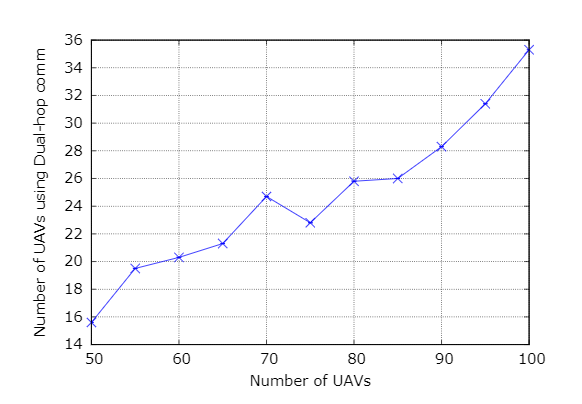
\includegraphics[scale=0.4]{rp6_Fig_6.png}
    \caption{Evaluation of the number of UAVs using Dual-Hop Communication }
    \label{fig:Number of UAV using Dual-Hop}
\end{figure}
\end{frame}

\begin{frame}{Conclusion}
\begin{itemize}
    \item One challenging problem in cellular UAVs is to cope with the massive data generated by these vehicles which could lead to decreased QoS.
    \item We addressed the issue of selecting the efficient communication strategy for UAVs.
    \item We considered a communication model that accounts for most propagation phenomena and derived the expression for effective rate for two strategies - \textbf{Direct communication} and \textbf{Dual-Hop communication}.
    \item We proposed a solution for selecting for each UAV the communication strategy providing better effective rate.
    \item We also discussed the efficiency of proposed solution through simulation graphs.
\end{itemize}
\end{frame}

\end{document}

